
\chapter{Theoretical Background}

There are different types of machine learning algorithms which have various application cases. In this case, an algorithm which performs object detection is used. In the following, the open source architecture YOLO (you only look once) is presented. First, the general principle of object detection is introduced, followed by the description of the architecture of deep YOLO networks. The principle of object detection is to combine Classification with detecting the boundaries of class instances which is exactly what needs to be done in the preprocessing step of sugar beet plants. By detecting the object boundaries of those plants, the image can be cropped to the right size which results in a standardized image format for the following regression task predicting the value of the damage (between 0 and 1).

The state of the art architecture for object detection is YOLO which was first introduced by \cite{yolov1}. Since then, two improved versions were published by the original author. These architectures were called YOLOv2 \cite{yolov2} and YOLOv3 \cite{yolov3}. After that, other authors published the next Version YOLOv4 \cite{yolov4} and also a newest version YOLOv5 can be found. 

The advantage of YOLO-networks is that they are much faster than other object detection algorithms like for example R-CNNs \cite{RCNN} which let the model run on a very high number of regions in the image. The idea of YOLO is that the network runs once for the complete image, predicting the bounding boxes and corresponding classes at once. It finds regions in the image which are assigned predicted bounding boxes and probabilities. In the following, the general idea of YOLO is introduced, followed by the incremental improvements in the following versions. 

\section{General Architecture of YOLO}
As proposed in the first introduction to YOLO in \cite{yolov1}, the network is designed to find objects and the corresponding boxes in a global manner meaning that the image is processed as whole once. Therefore, a $ S \times S $ grid divides the image into smaller parts. Each of those cells is responsible to predict $ B $ bounding boxes and corresponding confidences. This confidence is defined as $ Pr(Object) * IOU_{pred}^{truth} $. The bounding boxes consist of five predictions each, $ x, y, w, h $ and the confidence. The first four numbers represent the bounding box with the coordinates of the center $ (x,y) $ and the width and height (both relative to the whole image). Additionally, the cell predicts $ Pr(Class_i|Object) $, which are the conditional class probabilities. Only one set of class probabilities are predicted per cell. All in all, the the class probabilities and box confidence predictions are multiplied resulting in the class-specific confidence scores for each box: $ Pr(Class_i|Object) * Pr(Object) * IOU_{pred}^{truth} = Pr(Class_i) * IOU_{pred}^{truth} $.
 
\begin{figure}[htb!]
	\centering
	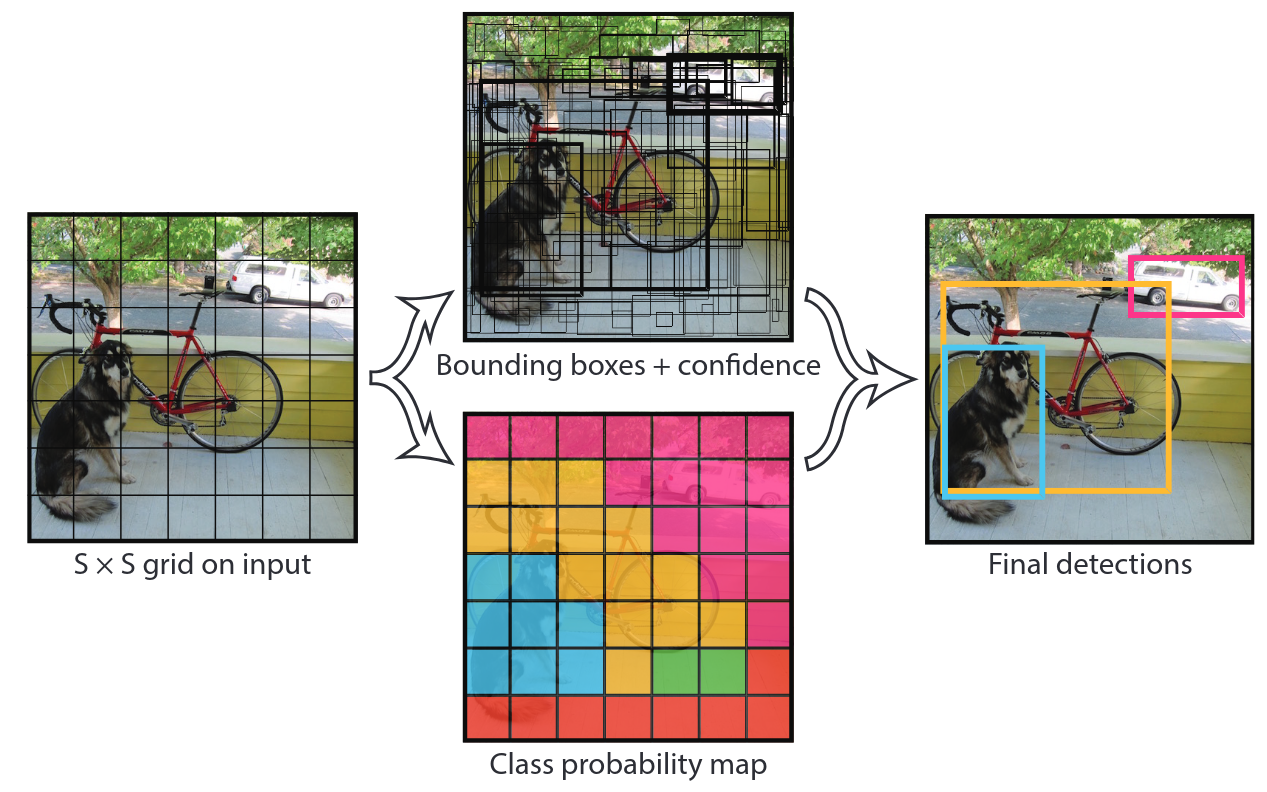
\includegraphics[scale=0.25]{figures/YOLO_functionality.png}
	\caption{Description of idea of YOLO. Taken from \cite{yolov1}}
	\label{fig:YOLO_idea}
\end{figure}

All in all, a tensor of size $ S \times S \times (B * 5 + C) $ results. Figure \ref{fig:YOLO_idea} depicts the idea of predicting bounding boxes with corresponding classes. \\

To achieve this, a convolutional neural network is used in combination with fully connected layers. The first part extracts features while the latter part predicts the probabilities and coordinates of the bounding boxes. It consists of 24 convolutional layer and 2 fully connected ones. The concrete network can be seen in figure \ref{fig:YOLO_network}. \\


\begin{figure}[htb!]
	\centering
	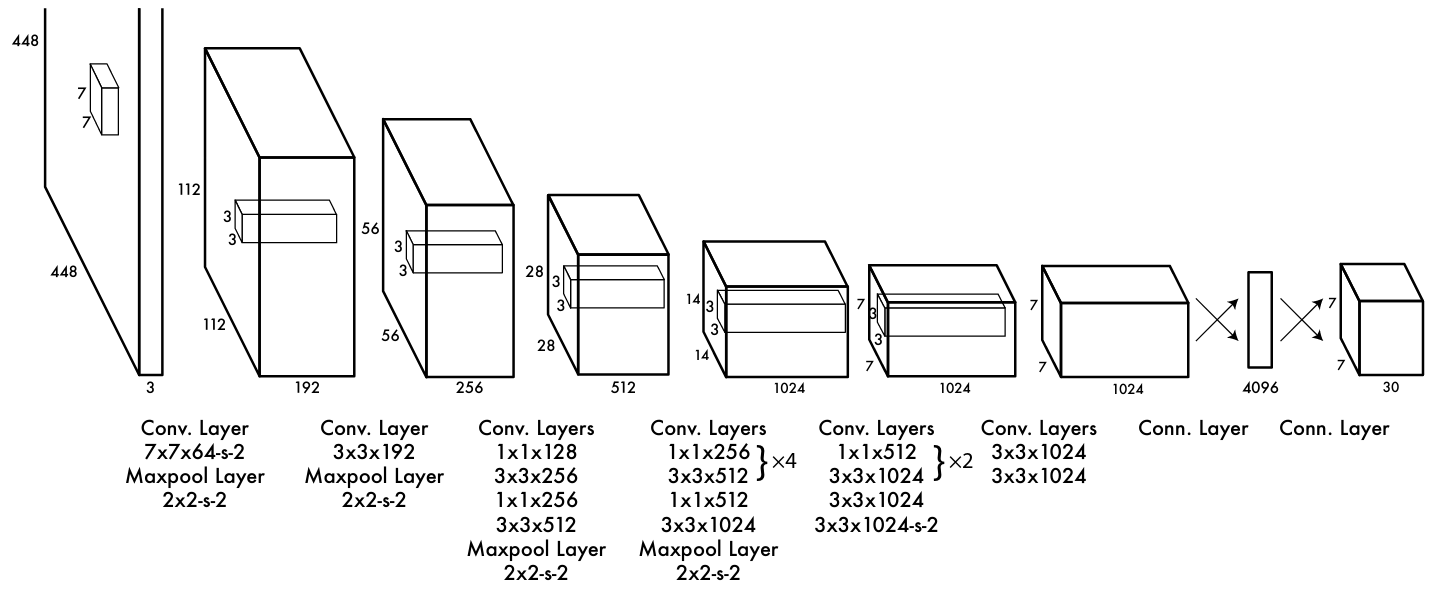
\includegraphics[scale=0.28]{figures/YOLO_network.png}
	\caption{Description of network of YOLO. Taken from \cite{yolov1}}
	\label{fig:YOLO_network}
\end{figure}

All in all, the first network has comparable accuracies as other object detection algorithms such as R-CNN or Fast R-CNN. The most important advantage of this architecture is the real time capability. Especially for this preprocessing task, the time plays an important role. 

\section{Incremental Improvements}

The first architecture was improved incrementally in different versions. The original authors were involved until version 3 (\cite{yolov1, yolov2, yolov3}). After that, other authors published improvements as YOLOv4 \cite{yolov4}. There is no publication to YOLOv5 yet, although there is already an implementation \cite{yolov5}. \\

\paragraph{YOLOv2}
With the first improvement which is published in \cite{yolov2}, the problem of the localization errors of the boundaries of objects are addressed. The authors call it a better, faster, and stronger version of the YOLO network because of the following improvements.

Depending on the authors, it is made better regarding the recall and localization of bounding boxes. The added batch normalization helps in regularization of the model. The dropout from the model can be left out without overfitting. It is also made better in terms of the image resolution. First, it is trained with the full resolution of $ 448 \times 448 $ for 10 epochs. Afterwards, the network is fine tuned on detection. Additionally, the last layers which were originally fully connected ones, are replaced by anchor boxes for the prediction of the bounding boxes. A disadvantage of doing this is that the box dimensions are hand picked. By running k-means clustering on the training set bounding boxes, it can be avoided and good priors can be found automatically. A second disadvantage of using anchor boxes is the instability of the model due to the coordinates of the centers of the boxes. These are calculated depending on the predicted box boundaries. Instead, it is better to predict the location coordinates relative to the cell's location resulting in values between 0 and 1. Another change is that the feature map is made finer so that the predictions get more accurate. One last change to make the network better is that multi-scale training. Due to the use of convolutional and pooling layers, the input resolution of images can easily be changed. This is used in the training to vary this resolution every few epochs. It makes it all in all more robust and not depending on the input resolution.

Additionally to making the network better, it is also made faster. The authors therefore introduce a new network called darknet-19 as the basis for YOLOv2. It has many advantages compared tp the previous one such as high accuracy and faster times. 

To make the network stronger, hierarchical classification is used. Therefore, the principle of subclassing is used. If a concrete dog such as Norfolk terrier is detected, it is also detected as Terrier and dog. Additionally, dataset combination with WordTree is used where multiple datasets are combined. With all this, joint classification and detection is possible meaning that classification and object detection datasets can be used to efficiently train the network.

All in all, this second version of YOLO already brings improvements to the network which is further made better in the next versions.


\paragraph{YOLOv3}
The main difference to YOLOv2 is that in the new version presented in \cite{yolov3}, a new network architecture for feature extraction is used. It is called Darknet-53 and the structure can be seen in figure \ref{fig:yolov3_architecture}.

\begin{figure}[htb!]
	\centering
	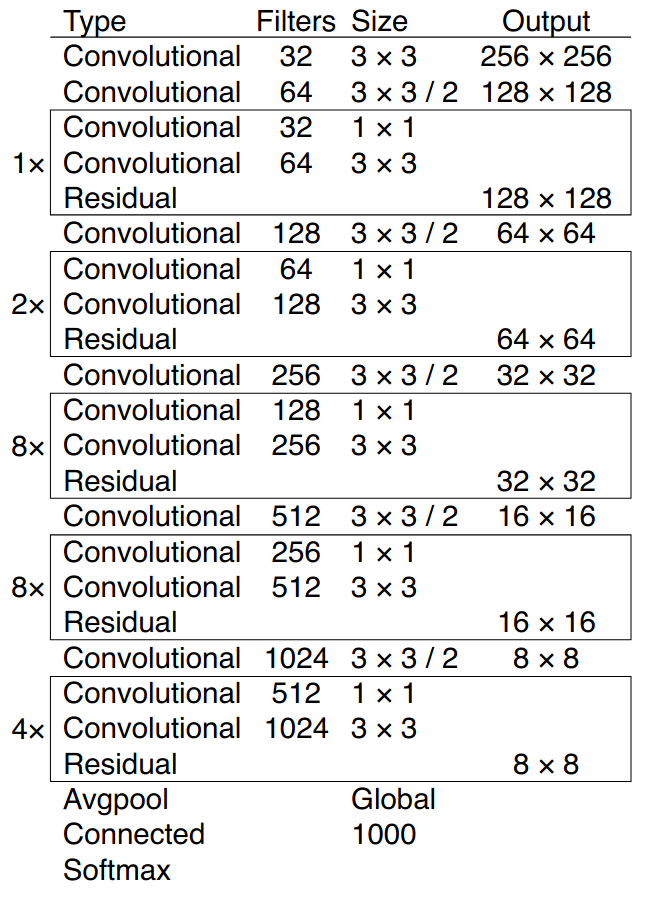
\includegraphics[scale=0.28]{figures/yolov3_architecture.png}
	\caption{Description of network of YOLOv3. Taken from \cite{yolov3}}
	\label{fig:yolov3_architecture}
\end{figure}

It is based on the architecture from YOLOv2 and Darknet-19 and has 53 convolutional layers. It is a deeper network, although the speeds are still much better than other comparable object detection models. 

The results show that the accuracy is comparable with ResNet-101 and ResNet-152, Top-5 is even best compared to the others. Additionally, the detectable frames per seconds are much higher than the other models.

\paragraph{YOLOv4}


Currently, many object detectors are built up in a similar way. The rough structure can be seen in figure \ref{fig:yolov4_architecture}.

\begin{figure}[htb!]
	\centering
	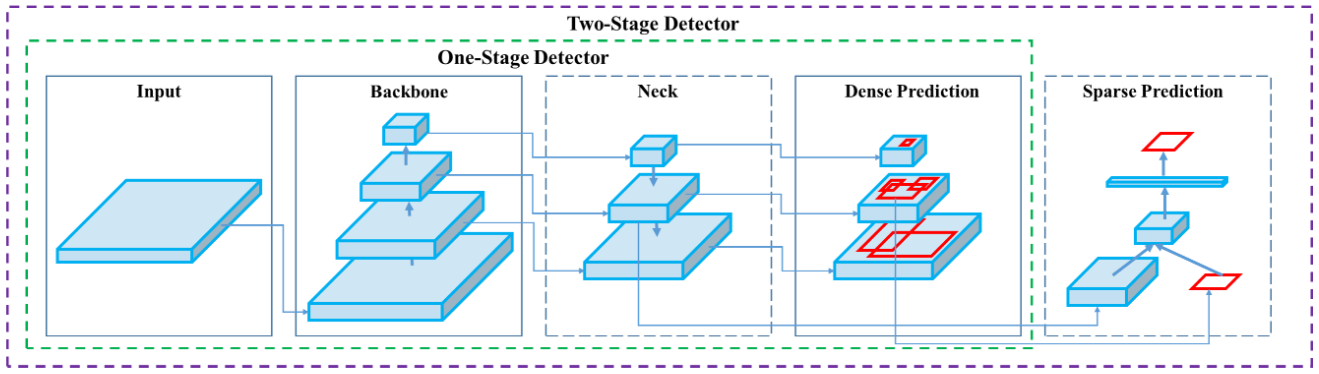
\includegraphics[scale=0.31]{figures/yolov4_architecture.png}
	\caption{Description of network of YOLOv4. Taken from \cite{yolov4}}
	\label{fig:yolov4_architecture}
\end{figure}

YOLOv4 \cite{yolov4} also consists of such parts. It is a One-Stage Detector and therefore only has dense prediction. As a backbone, CSPDarknet53 \cite{Wang_2020_CVPR_Workshops} is used. The neck consists of SPP (spatial pyramid pooling) \cite{7005506} and PAN (path aggregation network for instance segmentation) \cite{Liu_2018_CVPR}. Finally, the head (dense prediction) is the YOLOv3 network \cite{yolov3}. In addition, it uses some techniques such as data augmentation to improve accuracy for backbone and detector. 

All in all, the presented architecture with the additional techniques is superior to other state of the art object detection algorithms in both speed and accuracy. 

\section{Current Architecture YOLOv5} 

The current version YOLOv5 \cite{yolov5} again has further improvements compared to YOLOv4. The structure is similar to the previous one, also with the same backbone (CSPDarknet 53) and head (YOLOv3). One first difference is that instead of SPP, a faster version SPPF is used which is more than twice as fast. Together with PAN, this builds up the neck part.

\paragraph{Different Network Sizes}
There are five different network sizes available. They differ in the number of layers and parameters and are called YOLOv5n (nano, smallest), YOLOv5s (small), YOLOv5m (medium), YOLOv5l (large) and YOLOv5x (extra large). Additionally, each of the models 

\paragraph{Additional Features}
As data augmentation, different techniques are used. For example mosaic concatenates several images to one big image. The copy paste technique copies objects from images to other pictures.  Additionally, random affine transformations are applied to the images, such as rotations, scaling, translation and shear. Similar to mosaic, MixUp combines different images but with the difference that the pictures are directly laid behind each other. Additional settings like hue, saturation and value are randomly adjusted. Together with random horizontal flips, the variety of the training set is increased which leads to better object detection accuracy.
